
% % % % % % % % % % % % % % % % % % % % % % % % % % % % % % % % % %
%\documentclass[runningheads]{llncs}
\documentclass[preprint,10pt]{sigplanconf}

% packages
\usepackage{xspace}
\usepackage{ifthen}
\usepackage{amsbsy}
\usepackage{amssymb}
\usepackage{balance}
\usepackage{booktabs}
\usepackage{graphicx}
\usepackage{multirow}
\usepackage{needspace}
\usepackage{microtype}
\usepackage{bold-extra}
\usepackage{array}
\usepackage{epstopdf}



% references
\usepackage[colorlinks]{hyperref}
\usepackage[all]{hypcap}

\setcounter{tocdepth}{2}
\hypersetup{
	colorlinks=true,
	urlcolor=black,
	linkcolor=black,
	citecolor=black,
	plainpages=false,
	bookmarksopen=true}

\def\chapterautorefname{Chapter}
\def\appendixautorefname{Appendix}
\def\sectionautorefname{Section}
\def\subsectionautorefname{Section}
\def\figureautorefname{Figure}
\def\tableautorefname{Table}
\def\listingautorefname{Listing}

% source code
\usepackage{xcolor}
\usepackage{textcomp}
\usepackage{listings}
\definecolor{source}{gray}{0.9}
\lstset{
	language={},
	% characters
	tabsize=3,
	upquote=true,
	escapechar={!},
	keepspaces=true,
	breaklines=true,
	alsoletter={\#:},
	breakautoindent=true,
	columns=fullflexible,
	showstringspaces=false,
	basicstyle=\footnotesize\ttfamily,
	% background
	frame=single,
    framerule=0pt,
	backgroundcolor=\color{source},
	% numbering
	numbersep=5pt,
	numberstyle=\tiny,
	numberfirstline=true,
	% captioning
	captionpos=b,
	% formatting (html)
	moredelim=[is][\textbf]{<b>}{</b>},
	moredelim=[is][\textit]{<i>}{</i>},
	moredelim=[is][\color{red}\uwave]{<u>}{</u>},
	moredelim=[is][\color{red}\sout]{<del>}{</del>},
	moredelim=[is][\color{blue}\underline]{<ins>}{</ins>}}
\newcommand{\ct}{\lstinline[backgroundcolor=\color{white},basicstyle=\footnotesize\ttfamily]}
\newcommand{\lct}[1]{{\small\tt #1}}

% tikz
% \usepackage{tikz}
% \usetikzlibrary{matrix}
% \usetikzlibrary{arrows}
% \usetikzlibrary{external}
% \usetikzlibrary{positioning}
% \usetikzlibrary{shapes.multipart}
% 
% \tikzset{
% 	every picture/.style={semithick},
% 	every text node part/.style={align=center}}
% \tikzexternalize[prefix=figures/]{quality}

% proof-reading
\usepackage{xcolor}
\usepackage[normalem]{ulem}
\newcommand{\ra}{$\rightarrow$}
\newcommand{\ugh}[1]{\textcolor{red}{\uwave{#1}}} % please rephrase
\newcommand{\ins}[1]{\textcolor{blue}{\uline{#1}}} % please insert
\newcommand{\del}[1]{\textcolor{red}{\sout{#1}}} % please delete
\newcommand{\chg}[2]{\textcolor{red}{\sout{#1}}{\ra}\textcolor{blue}{\uline{#2}}} % please change
\newcommand{\chk}[1]{\textcolor{ForestGreen}{#1}} % changed, please check

% comments \nb{label}{color}{text}
\newboolean{showcomments}
\setboolean{showcomments}{true}
\ifthenelse{\boolean{showcomments}}
	{\newcommand{\nb}[3]{
		{\colorbox{#2}{\bfseries\sffamily\scriptsize\textcolor{white}{#1}}}
		{\textcolor{#2}{\sf\small$\blacktriangleright$\textit{#3}$\blacktriangleleft$}}}
	 \newcommand{\version}{\emph{\scriptsize$-$Id$-$}}}
	{\newcommand{\nb}[2]{}
	 \newcommand{\version}{}}
\newcommand{\rev}[2]{\nb{Reviewer #1}{red}{#2}}
\newcommand{\ab}[1]{\nb{Alexandre}{blue}{#1}}
\newcommand{\sv}[1]{\nb{Santiago}{orange}{#1}}
\newcommand{\TG}[1]{\nb{TG}{magenta}{#1}}

% graphics: \fig{position}{percentage-width}{filename}{caption}
\DeclareGraphicsExtensions{.png,.jpg,.pdf,.eps,.gif}
%\graphicspath{{figures/}}
\newcommand{\fig}[4]{
	\begin{figure}[#1]
		\centering
		\includegraphics[width=#2\textwidth]{#3}
		\caption{\label{fig:#3}#4}
	\end{figure}}
\newcommand{\largefig}[4]{
	\begin{figure*}[#1]
		\centering
		\includegraphics[width=#2\textwidth]{#3}
		\caption{\label{fig:#3}#4}
	\end{figure*}}

% abbreviations
\newcommand{\ie}{\emph{i.e.,}\xspace}
\newcommand{\eg}{\emph{e.g.,}\xspace}
\newcommand{\etc}{\emph{etc.}\xspace}
\newcommand{\etal}{\emph{et al.}\xspace}

% lists
\newenvironment{bullets}[0]
	{\begin{itemize}}
	{\end{itemize}}

\newcommand{\seclabel}[1]{\label{sec:#1}}
\newcommand{\secref}[1]{Section~\ref{sec:#1}\xspace}
\newcommand{\figlabel}[1]{\label{fig:#1}}
\newcommand{\figref}[1]{Figure~\ref{fig:#1}\xspace}

\usepackage{subfig}
\DeclareCaptionType{copyrightbox}
% D O C U M E N T
% % % % % % % % % % % % % % % % % % % % % % % % % % % % % % % % % %
\begin{document}

% T I T L E
% % % % % % % % % % % % % % % % % % % % % % % % % % % % % % % % % %

\title{Extending Mondrian with Interactive HTML Visualisation}

\authorinfo{Santiago Vidal}
	{ISISTAN Research Institute, Faculty of Sciences, UNICEN University, Campus Universitario, Tandil, Buenos Aires, Argentina, Also CONICET}
	{svidal@exa.unicen.edu.ar}
\authorinfo{Alexandre Bergel}
	{PLEIAD Lab, Department of Computer Science (DCC), University of Chile, Santiago, Chile}
	{http://bergel.eu}
\authorinfo{Claudia Marcos} 
	{ISISTAN Research Institute, Faculty of Sciences, UNICEN University, Campus Universitario, Tandil, Buenos Aires, Argentina, Also CIC}
	{cmarcos@exa.unicen.edu.ar}
\authorinfo{Tudor G\^irba} 
	{netstyle.ch GmbH, Switzerland}
	{tudor@tudorgirba.com}


\maketitle

% A B S T R A C T
% % % % % % % % % % % % % % % % % % % % % % % % % % % % % % % % % %

%\begin{abstract}
%\end{abstract}

%: % % % % % % % % % % % % % % % % % % % % % % % % % % % % % % % % %
\TG{I think it is hard to find anything scientific in this work. One idea is to position it as a tool demo (\ie engineering work). In any case, we need to describe the cases that posed a challenge. The angle can be that you basically built a transformation between the graph model of Mondrian and the model of Protovis.}

\TG{The only contribution is that it is available on the browser. It is not scientific, just engineering. However, we can talk about the challenges of transforming the model of Mondrian in the model of Protovis. For example, we can talk about the problem of arranging the nodes / edges in layers, the scoping of drag and drop}

\section{Introduction}\seclabel{introduction}

Mondrian~\cite{Meye06a} is an agile visualization engine primarily used to visualize software\footnote{\url{http://www.moosetechnology.org/tools/mondrian}}. Mondrian support vectorial rendering made of primitive geometrical objects. Mondrian is built in Pharo and use Morphic canvas to render a visualization.

We realized an experiment to render Mondrian visualizations in a web browser. This paper presents the exporter we built for Protovis\footnote{\url{http://vis.stanford.edu/protovis}}~\cite{Bost09a}, a Javascript graphical toolkit for data visualization.

%problem

%solution

%surprising result

%contribution

%\item lesson learnt

%outline
The paper is structured as follows.

%\secref{problem} shows the problem we faced when trying to evolve Mondrian.
%\secref{refactoring} describes the aspect-based solution we adopted.
%\secref{results} presents the impact of our solution on Mondrian.
%\secref{relatedWork} briefly revise the related work.
%\secref{conclusion} concludes.


%: % % % % % % % % % % % % % % % % % % % % % % % % % % % % % % % % %
%\section{Refactoring Mondrian to Enable the Extensions}\seclabel{problem}
%
%Implementation of the visitor pattern instead of the displayOn: methods
%Show some benchmarks. We have they in a mail with the subject bench

\section{Protovis} \seclabel{protovis}
Protovis is a visualization toolkit written in JavaScript that enables the creation of complex and interactive graphics in web-browsers without the need of an extra plugin. The data to be visualized is defined by means of simple marks such as bars, lines and dots. 

Protovis makes intensive use of a fluent interface, intended to build readable code. For example, the following script defines a bar of \ct{height=100} and \ct{width=20} (\figref{SimpleBar2}) with a label:

\begin{lstlisting} 
new pv.Panel().width(150).height(150)
  .add(pv.Bar)
    .data([100])
    .left(10).bottom(0)
    .width(20).height(function(d) d)
  .add(pv.Label)
    .left(30).bottom(50)
    .text("Simple Visualization")
  .root.render();
\end{lstlisting}

In this example, the  \ct{left} and \ct{bottom} define the panel position \ct{x,y} in which the figure is drawn.

\fig{h}{0.2}{SimpleBar2}{Example in Protovis.}

%\begin{figure}
%\begin{center}
%\begin{raggedright}
%
\includegraphics[bb=20bp 743bp 100bp 812bp,scale=0.99]{SimpleBar} 
%\par\end{raggedright}
%\end{center}
%\caption{Simple Visualization with Protovis.\label{fig:SimpleBar}}
%\end{figure}  

%: % % % % % % % % % % % % % % % % % % % % % % % % % % % % % % % % %
\section{Generating HTML Files using a Visualization Library}\seclabel{generating}

Given a view generated with Mondrian we want to be able to export it to an HTML file using the Protovis toolkit. In addition of obtaining a similar visualization graph, a support for interaction is required. 

The generation of HTML files with Protovis visualizations in Mondrian involves two main steps: (1) the creation of the dataset that contains information on which to base the graph, and (2) the description of the marks to be drawn. The accomplishment of these steps is detailed in the following sections.

\subsection{Generating the Datasets}
The standard way to send data to Protovis is by means of a JSON (JavaScript Object Notation) descriptions. Owing to the components to be exported are currently drawn in the Mondrian canvas, the dataset description must be inferred from it\ab{I do not understand this sentence}. As the canvas data is represented by mean of the \ct{MOGraphElement} hierarchy, the dataset description is created through a Visitor pattern~\cite{Gamm95a} as shown in Figure \ref{fig:VisitorPattern}.

\begin{figure}
\begin{centering}
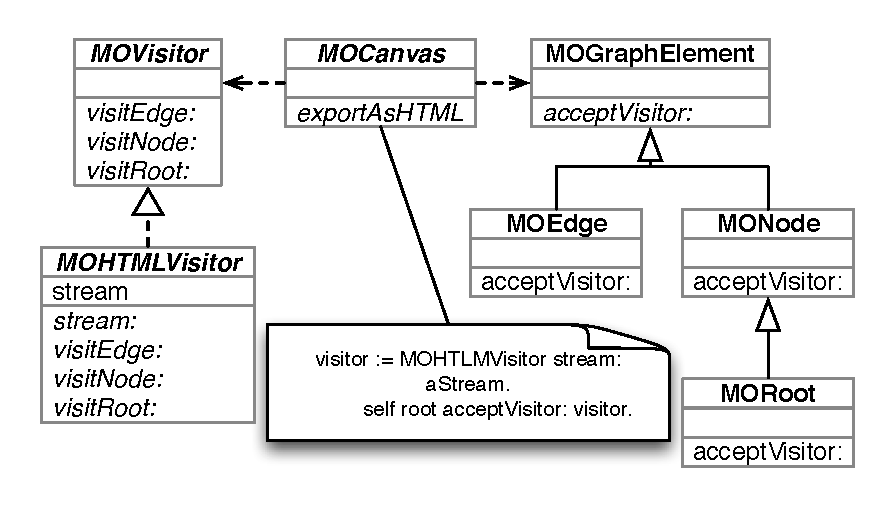
\includegraphics[bb=0bp 0bp 413bp 228bp,scale=0.60]{VisitorPattern} 
\par\end{centering}

\caption{Visitor Pattern.\label{fig:VisitorPattern}}

\end{figure}
The JSON structure that we generate is created from the nodes and edges composing the Mondrian view. For this reason the structure \ab{Which structure? The structure generated by our exporter written in JSON?} contains two arrays: nodes and links. The former contain a collection of objects that represent nodes by means of information that allows its correct visualization with Protovis. For example, given the next JSON object a node is specified
\begin{lstlisting} 
{
 nodeID:0, nodeShape:"a MORectangleShape", 
 nodeName:"CharacterSet", 
 nodeWidth:5.0, nodeHeight:18, 
 x:5.0, y:241, 
 nodeFillColor:"#F8F8F8", nodeBorderColor:"#000000", 
 nodeType:"parent"
}
\end{lstlisting}
where \ct{nodeID} is a number that identifies a node uniquely. The variable \ct{nodeShape} indicates the kind of shape that must be drawn (in this case a rectangle). Other possible shapes include circle, label and a bitmap image. The variable \ct{nodeName} contains the text to be displayed by the tooltip of the node. The size of a shape is indicated by \ct{nodeWidth} and \ct{nodeHeight}. The variables \ct{x} and \ct{y} are used to know the position of the canvas in which the node will be displayed. The fill and border colors of a node are indicated through the variables \ct{nodeFillColor} and \ct{nodeBorderColor}. Finally, the variable \ct{nodeType} indicates if the node is a leaf on a hierarchy or not. This variable is used for interaction purposes.
\sv{I don't know if this is clear. I used this variable to redraw correctly after a drag and drop interaction. For example, if a parent node is dragged in a DistributionMap graph, the children must be redrawn accordingly} \ab{I think it is okay for now}

Regarding the links, their structure is simpler than the nodes. Consider the following example in which a link is defined:
\begin{lstlisting} 
{
 sourceID:1, 
 targetID:19,
 edgeColor:"#9F9F9F",
}
\end{lstlisting}

This object defines a link between the nodes whose IDs are 1 and 19 respectively. Also, the color of the link is specified by the object. 

All the data needed to the generation of the dataset is taken from the classes \ct{MOEdge}, \ct{MONode}, and \ct{MORoot} when the visitor pattern runs through them iteratively.

%\sv{Explain the implementation of the Visitor pattern that collects the data to generate the HTML file.}

\subsection{Describing the Marks}

Once the dataset is generated, the Protovis JavaScript code that creates the visualization of the different kind of marks must be described. This process comprises: 
\begin{itemize}
\item Creation of the Protovis canvas
\item Description of the marks to be drawn (nodes and links)
\item Interaction behavior
\item Layout specification
\item Tooltip creation
\end{itemize}

The Protovis canvas is initially created with the same size as the canvas of Mondrian. However, it is automatically resized when a dragging operation is detected out of it.

As Protovis uses a declarative syntax each kind of mark is declared once \TG{What does ``declared once'' mean? It would be declared once no matter what :)}. \ab{I do not understand the remaining of the section} This is different only for lines which are declared individually for each link of the dataset. In this way to visualize nodes whose shape is \ct{MORectangleShape} the next code must be declared once \ab{What the following code does?}\ab{What about adding a screenshot?}
\begin{lstlisting} 
vis.add(pv.Bar)
   .data(getNodesByShape("a MORectangleShape"))
   .fillStyle(function(d) d.nodeFillColor)
   .strokeStyle(function(d) d.nodeBorderColor)
   .width(function(d)d.nodeWidth)
   .height(function(d)d.nodeHeight)
   .left(function(d) d.nodeType=="parent" ? d.x : (dataset.nodes[d.nodeParentID].x+d.x))
   .top(function(d) d.nodeType=="parent" ? d.y : (dataset.nodes[d.nodeParentID].y+d.y))
   .text(function(d)d.nodeName)
   .event("mouseover", pv.Behavior.tipsy2({html: true}))
   .event("mousedown", pv.Behavior.drag2());
\end{lstlisting}

As can be seen, in order of visualize a rectangular shape a Bar mark is used. The call to \ct{getNodesByShape}, inside the \ct{data} method, is used to retrieve only those nodes whose shape is \ct{MORectangleShape}. In regard to the following two methods \ct{fillStyle} and \ct{strokeStyle} they set the fill and border colors of the shape using the values found in the node declaration in the dataset. The size of the figure is also defined using the values of the dataset through the methods \ct{width} and \ct{height}.

Regarding the position in which a shape is drawn this is accomplished by mean of the methods \ct{left} and \ct{top} and the values defined in the node object. That is, the layout used to generate the HTML file is the same used by Mondrian. However, the \ct{x,y} values are defined depending on the kind of \ct{nodeType}. When \ct{nodeType =='children'} the position of the node is determined using the father's position. This kind of definition is specially useful when a parent node is changed of position because the child nodes can be dynamically updated accordingly.  

The last 3 methods deal with interaction. The \ct{text} method sets the string that would be displayed as a tooltip. This behavior is accomplished by using an external tooltip library called Tipsy \footnote{\url{http://onehackoranother.com/projects/jquery/tipsy}}. It was chosen because it supports HTML code which makes possible different formats of text shown in the tooltip. 

Finally, the last \ct{event} method handles the drag and drop interaction over a node. Although, Protovis defines a standard drag interaction it was rewritten in order to improve the performance during dragging a node. That is,  only the node dragged is redrawn during a dragging operation, as well as the child nodes of it. This interaction handler also controls the children nodes position.For example, if a node is an inner node, its position is limited to the perimeter of the parent node.

The declaration of the visualization of a link is simpler than a node declaration. Consider the following code 
\begin{lstlisting} 
vis.add(pv.Line)
   .data(function() getPoints(dataset.links[0]))
   .left(function(d) d.x)
   .top(function(d) d.y)
   .strokeStyle(dataset.links[0].edgeColor);
\end{lstlisting}
In this case the link is defined by a \ct{Line} mark. The data is generated through the \ct{getPoints} method with has the first link object of the dataset as a parameter. As was said, for each link object of a dataset one of this definitions is made. The \ct{getPoints} method calculates the \ct{x,y} positions of the beginning and end of the link. This position values are used to set the \ct{left} and \ct{top} methods. Finally, the color of the link is selected by means of \ct{strokeStyle} according to the value of the link object.

\subsection{Supported Graphs}

%To properly visualize the exported graphs some additional files are needed such as the Protovis library or interaction handler files. However, this need is transparent for the users because the exporter created these files when they are needed. This was implemented by means of packaging the additional files in a compressed file and then creating a binary code of them through \ct{Base64MimeConverter}. So, when an HTML file is exported, the compressed file is decoded an extracted in the same directory than the HTML file. 

Currently the export method to HTML files with Protovis supports all the Mondrian visualizations composed by graphics elements such as rectangles, lines, and labels. Examples of this kind of visualizations are distribution maps, inner nodes, blueprint classes or system complexity. 

\ab{Ok, but what are the limitations? Why Hapao cannot be exported?}

%For example a system complexity visualization shows the inheritance relationships between classes. The classes are represented through rectangles and the inheritance relationships are represented through lines (Figure \ref{fig:SistemComplexityMondrianEasel}). Additionally, the size of a class is represented by means of its height (number of methods), its width(number of attributes), and its color (number of lines of code). When this visualization is exported to an HTML file using Protovis the process described in the previous sections is run. So, a dataset and Protovis marks are described and the file is generated producing a similar visualization as is shown in Figure \ref{fig:SistemComplexityHTML}.

%\begin{figure*}
%\subfloat[Mondrian]{\label{fig:SistemComplexityMondrianEasel}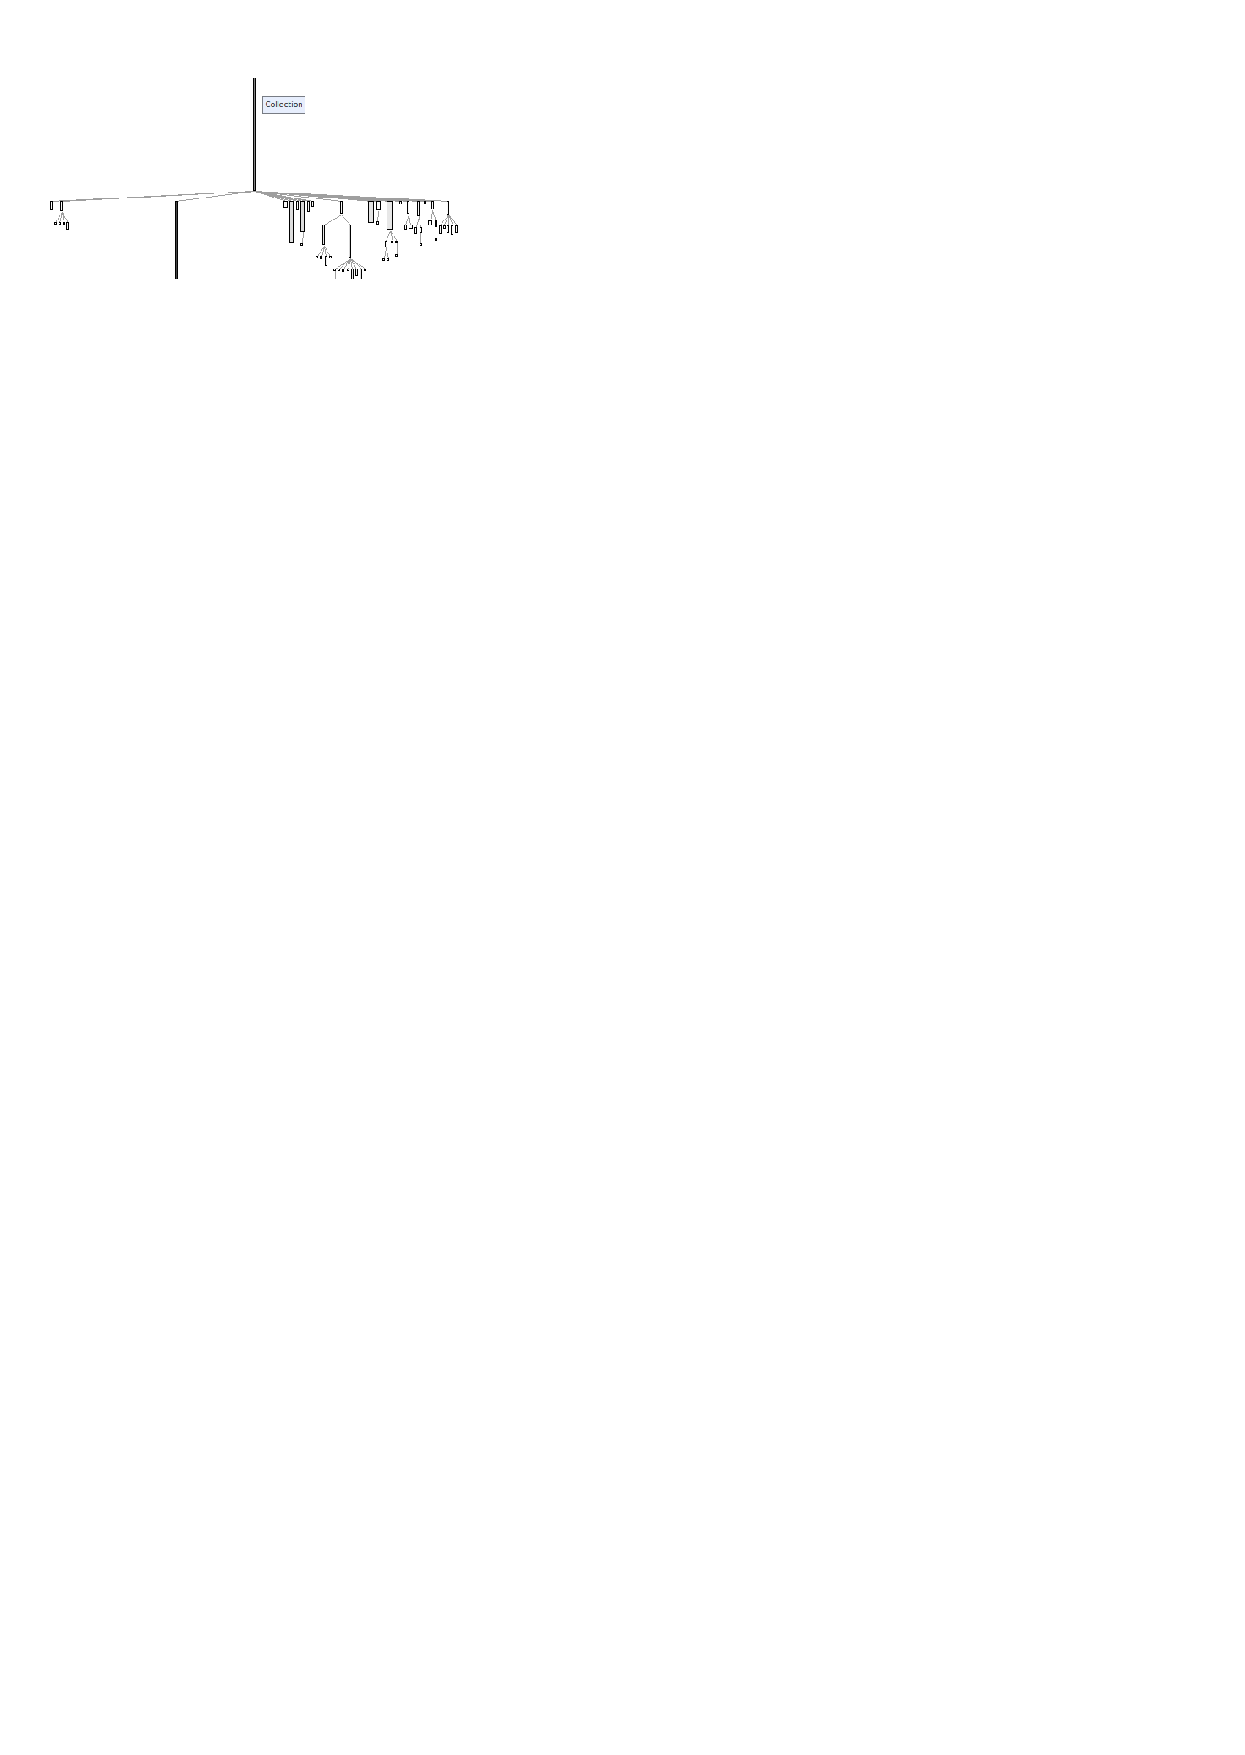
\includegraphics[bb=15bp 700bp 225bp 810bp,clip,scale=0.95]{SistemComplexityMondrianEasel}
%
%}\subfloat[HTML]{\label{fig:SistemComplexityHTML}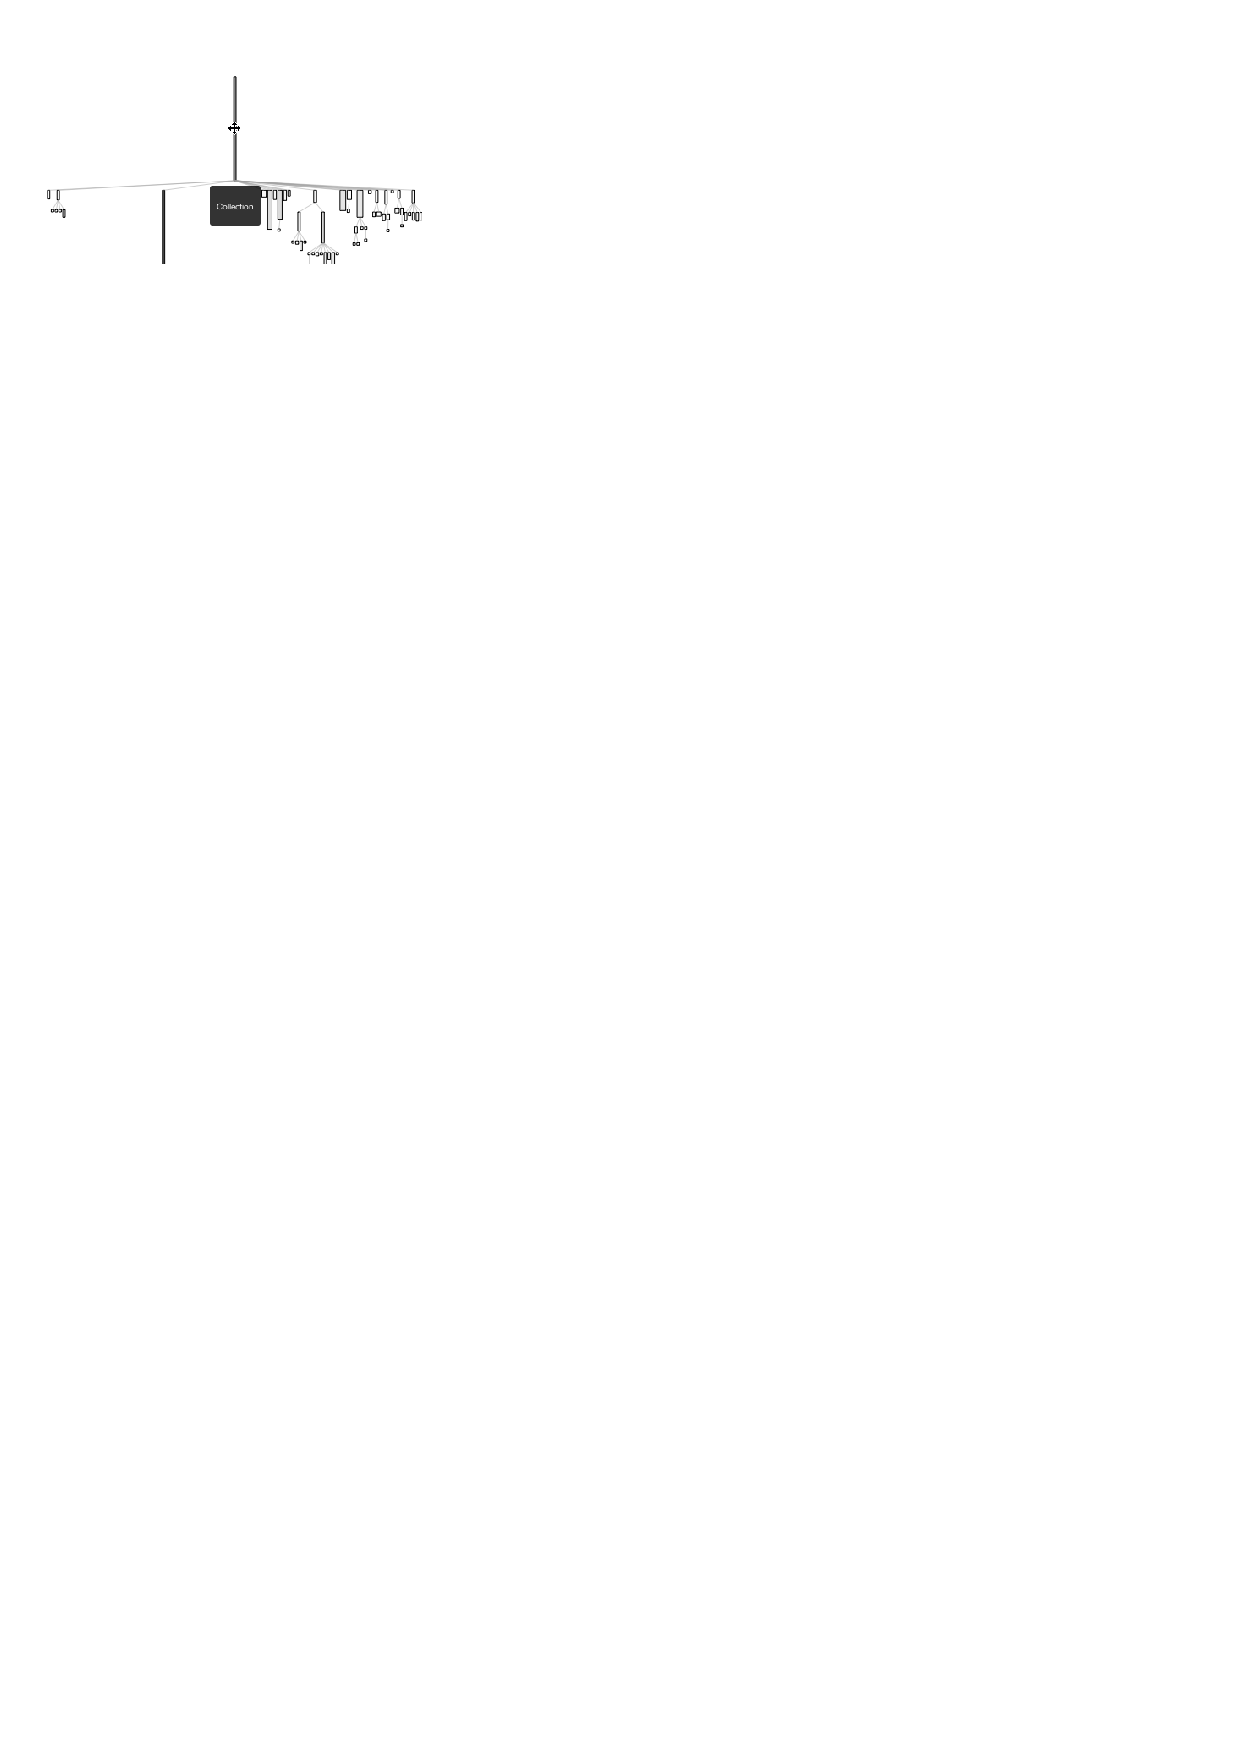
\includegraphics[bb=15bp 710bp 210bp 810bp,clip]{SistemComplexityHTML}
%
%}
%
%\caption{Visualization of system complexity}
%
%\end{figure*}


%\ab{We need some example. For example, how do you translate ``view nodes: MOShape withAllSubclasses''}
%\ab{view shape rectangle height: \#numberOfMethods; width: \#numberOfAttributes. view nodes: MOShape withAllSubclasses}

%I used the layouts given by Mondrian
%I used Tipsy
%I reimplemented drag&drop
% Some things changed in the drag & drop implementation

%: % % % % % % % % % % % % % % % % % % % % % % % % % % % % % % % % %
\section{Future Works}\seclabel{results}

\paragraph{Dedicated layout and node description.} Protovis offers numerous layouts and graph representation. Mondrian should provide a class \ct{MOProtovisLayout}

\paragraph{Better interaction support.} \ab{What can be done in Protovis? Menu? Can new visualization be opened by clicking on a node?}

\paragraph{Exposure via Seaside.}
being behind a seaside server



%: % % % % % % % % % % % % % % % % % % % % % % % % % % % % % % % % %
\section{Conclusion}\seclabel{conclusion}



% % % % % % % % % % % % % % % % % % % % % % % % % % % % % % % % % %
%\section*{Acknowledgments}
%
%\small We gratefully thanks ...

% bibliography
% % % % % % % % % % % % % % % % % % % % % % % % % % % % % % % % %
\bibliographystyle{abbrvnat}
\bibliography{}

\end{document}
